% Компіляція: lualatex -shell-escape main.tex (двічі для змісту)
\documentclass[12pt,a4paper]{article}

\usepackage{fontspec}
\usepackage{polyglossia}
\setdefaultlanguage{ukrainian}
\setmainfont{NewComputerModern10}
\setsansfont{Noto Sans}
\setmonofont{Noto Sans Mono}[Scale=0.82]

\usepackage{
  amsmath,
  amssymb,
  array,
  booktabs,
  caption,
  enumitem,
  float,
  geometry,
  graphicx,
  microtype,
  titlesec,
  xcolor
}
\usepackage[newfloat]{minted}
\geometry{left=2cm,right=2cm,top=2cm,bottom=2cm}
\setlength{\parindent}{1.25cm}
\setlength{\parskip}{0pt}
\linespread{1.08}

\titleformat{\section}
  {\normalfont\fontsize{14}{16}\selectfont\bfseries\centering}
  {\thesection.}{0.6em}{}
\titleformat{\subsection}
  {\normalfont\fontsize{12}{14}\selectfont\bfseries\centering}
  {\thesubsection.}{0.6em}{}
\titlespacing*{\section}{0pt}{1.4em}{0.65em}
\titlespacing*{\subsection}{0pt}{1.1em}{0.45em}
\captionsetup{font=small,labelfont=bf,labelsep=endash}
\captionsetup[table]{position=bottom,skip=5pt}

\usemintedstyle{vs}
\setminted{linenos,breaklines,frame=single,fontsize=\scriptsize,tabsize=4}
\SetupFloatingEnvironment{listing}{name=Лістинг}

\usepackage[
  unicode,
  colorlinks=true,
  linkcolor=black,
  urlcolor=blue,
  pdftitle={ІО-41, Давидчук А. М., Технології Computer Vision, Лабораторна робота №1},
  pdfauthor={Давидчук Артем},
  pdfsubject={2D та 3D матричні геометричні перетворення}
]{hyperref}

\newcommand{\studentName}{Давидчук А. М.}
\newcommand{\studentGroup}{ІО-41}
\newcommand{\recordBook}{4106}
\newcommand{\teacherName}{Баран Д. Р.}
\newcommand{\reportYear}{2026}

\begin{document}

\pagenumbering{gobble}
\begin{titlepage}
  \begin{center}
    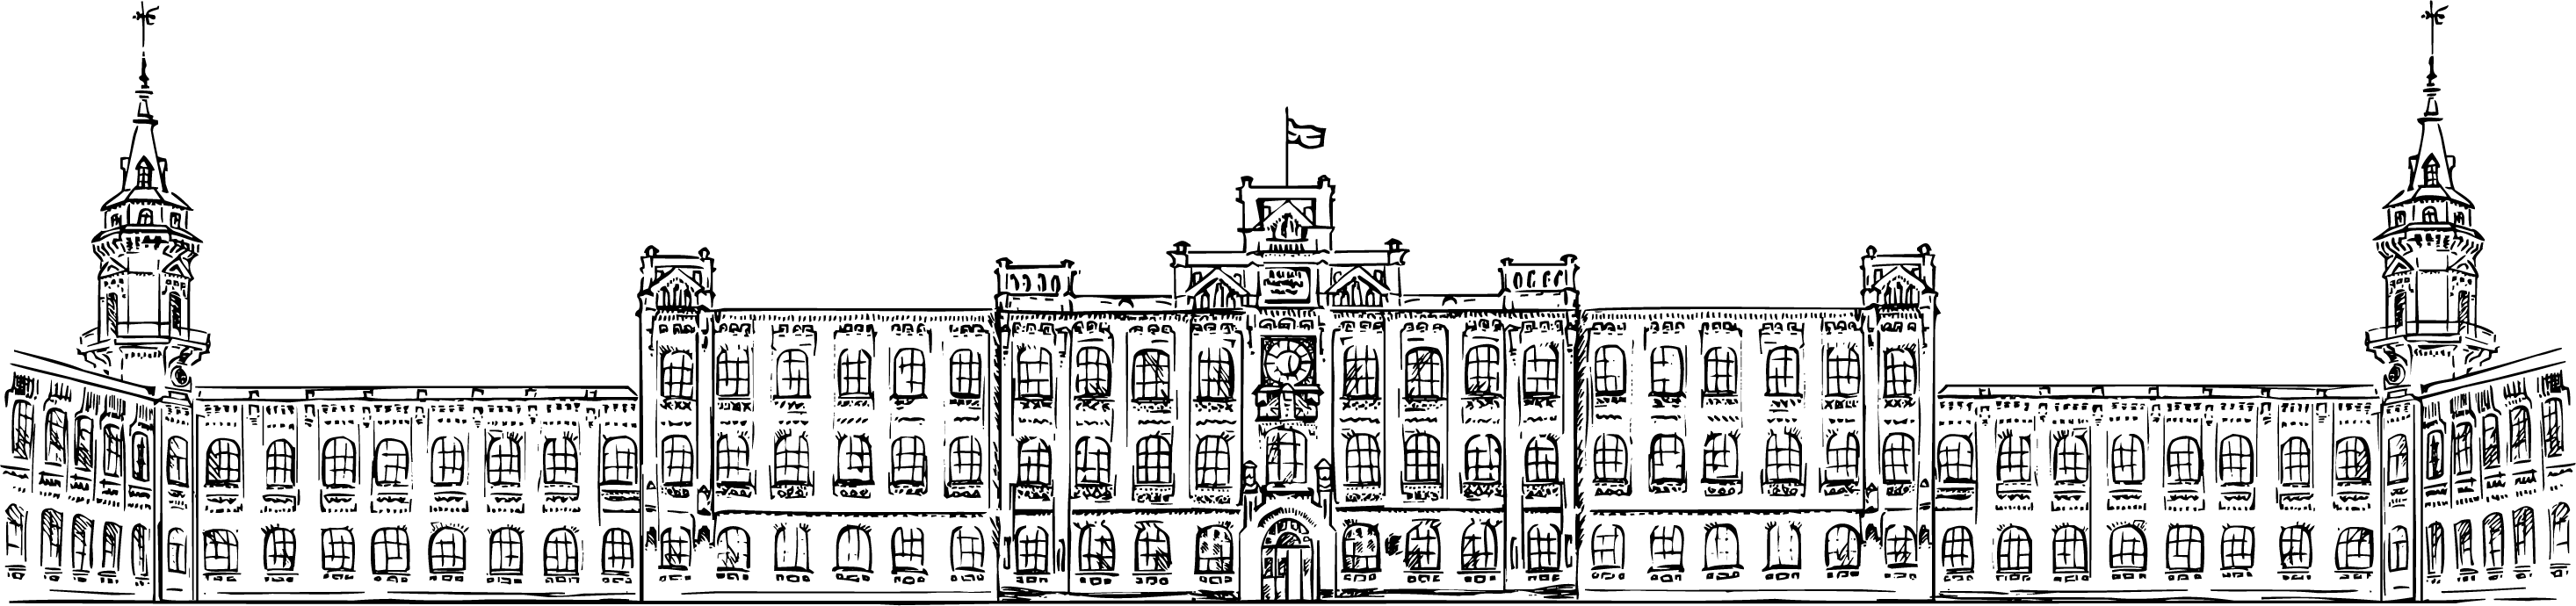
\includegraphics[width=0.7\textwidth]{../../../../../../templates/letterhead.png}
  \end{center}

  \begin{center}
    \large
    Національний технічний університет України\\
    «Київський політехнічний інститут імені Ігоря Сікорського»\\[1em]
    Факультет інформатики та обчислювальної техніки\\
    Кафедра обчислювальної техніки
  \end{center}

  \vfill

  \begin{center}
    \textbf{\LARGE Технології Computer Vision}\\[2em]
    \textbf{\Large Лабораторна робота №1}\\[0.7em]
    \parbox{0.9\textwidth}{\centering
      «Дослідження технологій побудови та перетворення координат площинних і просторових об’єктів»}
  \end{center}

  \vfill

  \begin{flushright}
    \begin{minipage}{0.48\textwidth}
      Виконав: студент 3 курсу ФІОТ,\\
      групи \studentGroup\\
      \textit{\studentName}\\
      Залікова книжка № \recordBook\\[1em]
      Перевірив: \textit{\teacherName}
    \end{minipage}
  \end{flushright}

  \vfill
  \begin{center}Київ --- \reportYear\end{center}
\end{titlepage}

\pagenumbering{arabic}
\setlength{\parindent}{0pt}

\section{Тема та мета роботи}

\noindent
\textbf{Тема:} дослідження технологій побудови та перетворення координат площинних і просторових об’єктів.

\medskip

\noindent
\textbf{Мета:} дослідити задання координат 2D- та 3D-геометричних об’єктів, реалізувати матричні переміщення, масштабування, обертання та проекцію, а також візуалізувати результати засобами Python, NumPy і Matplotlib.

\section{Завдання роботи}

Відповідно до варіанта 9 виконано дві частини лабораторної роботи:

\begin{itemize}[leftmargin=*,itemsep=0.25em]
  \item побудувати квадрат, реалізувати послідовність «переміщення + масштабування --- переміщення», виконати її циклічно та відобразити траєкторію зміни положення;
  \item побудувати піраміду з чотирикутною основою, виконати аксонометричну проекцію та циклічне обертання навколо внутрішньої осі, реалізувати появу і зникнення фігури зі зміною кольору контуру та заливки.
\end{itemize}

\section{Математична модель}

\subsection{2D-перетворення}

Вершини квадрата подано матрицею розширених координат, у якій кожен стовпець є окремою вершиною:

\begin{equation}
P=\begin{bmatrix}x_1&x_2&x_3&x_4\\y_1&y_2&y_3&y_4\\1&1&1&1\end{bmatrix}.
\end{equation}

Матриця переміщення має вигляд:

\begin{equation}
T(d_x,d_y)=\begin{bmatrix}1&0&d_x\\0&1&d_y\\0&0&1\end{bmatrix}.
\end{equation}

Масштабування навколо центра квадрата \(C=(c_x,c_y)\) реалізується композицією:

\begin{equation}
S_C=T(C)\,S\,T(-C), \qquad
S=\begin{bmatrix}s_x&0&0\\0&s_y&0\\0&0&1\end{bmatrix}.
\end{equation}

Загальна матриця для варіанта 9:

\begin{equation}
P'=T_2\,T(C)\,S\,T(-C)\,T_1\,P.
\end{equation}

У кожному кадрі початкова матриця квадрата використовується як еталон, а параметри \(T_1\), \(S\) і \(T_2\) змінюються відповідно до номера кадру.

\subsection{3D-перетворення та проекція}

Піраміда задається п’ятьма вершинами у розширених координатах:

\begin{equation}
P=\begin{bmatrix}x_1&\dots&x_5\\y_1&\dots&y_5\\z_1&\dots&z_5\\1&\dots&1\end{bmatrix}.
\end{equation}

Для обертання навколо внутрішньої вертикальної осі використано матрицю:

\begin{equation}
R_z(\theta)=\begin{bmatrix}
\cos\theta&-\sin\theta&0&0\\
\sin\theta&\cos\theta&0&0\\
0&0&1&0\\
0&0&0&1
\end{bmatrix}.
\end{equation}

Піраміда центрована відносно осі \(Z\), тому ця вісь проходить через її внутрішню область. Для отримання аксонометричного вигляду застосовано фіксований нахил навколо осей \(X\) та \(Y\), після чого координату \(Z\) відкинуто під час переходу до екрана:

\begin{equation}
P_{2D}=P_{XY}\,R_y(\alpha)\,R_x(\beta)\,R_z(\theta)\,P_{3D}.
\end{equation}

Тут \(R_z\) задає анімаційне обертання, \(R_x\) і \(R_y\) задають напрям спостереження, а \(P_{XY}\) виконує проекцію на площину екрана.

\section{Архітектура та алгоритми}

Програму розділено на функції створення об’єктів, побудови матриць, перетворення координат, проекції та візуалізації.

\begin{table}[H]
  \centering
  \renewcommand{\arraystretch}{1.2}
  \begin{tabular}{|p{6.2cm}|p{8.2cm}|}
    \hline
    \textbf{Компонент} & \textbf{Призначення} \\
    \hline
    \texttt{create\_square}, \texttt{create\_pyramid} & Формування матриць вершин. \\
    \hline
    \texttt{translation\_matrix}, \texttt{rotation\_*}, \texttt{scaling\_matrix} & Побудова однорідних матриць перетворень. \\
    \hline
    \texttt{transform\_square}, \texttt{transform\_pyramid} & Формування положення об’єкта для поточного кадру. \\
    \hline
    \texttt{project\_axonometric}, \texttt{project\_to\_screen} & Перехід від 3D до 2D та розміщення у вікні. \\
    \hline
    \texttt{FuncAnimation} & Циклічне оновлення координат, кольорів і прозорості. \\
    \hline
  \end{tabular}
  \caption{Компоненти програмного рішення}
\end{table}

\subsection{Алгоритм 2D-частини}

\begin{enumerate}[leftmargin=*,itemsep=0.25em]
  \item Створити початкову матрицю координат квадрата.
  \item Для поточного кадру обчислити перше переміщення.
  \item Знайти центр переміщеного квадрата.
  \item Виконати масштабування навколо центра.
  \item Застосувати друге переміщення.
  \item Оновити полігон квадрата та додати координати його центра до траєкторії.
\end{enumerate}

\subsection{Алгоритм 3D-частини}

\begin{enumerate}[leftmargin=*,itemsep=0.25em]
  \item Створити матрицю п’яти вершин піраміди та список її граней.
  \item Для кожного кадру обчислити кут обертання навколо осі \(Z\).
  \item Застосувати обертання та фіксований нахил навколо осей \(X\) і \(Y\).
  \item Відкинути координату \(Z\) і перевести результат у координати екрана.
  \item Оновити п’ять полігонів-граней.
  \item Змінити кольори контуру й заливки та коефіцієнт прозорості.
\end{enumerate}

\section{Структура проєкту}

У папці лабораторної роботи розміщено:

\begin{itemize}[leftmargin=*,itemsep=0.25em]
  \item \texttt{2D.py} --- реалізація 2D-перетворень квадрата та його анімації;
  \item \texttt{3D.py} --- реалізація піраміди, 3D-перетворень, проекції та анімації;
  \item \texttt{requirements.txt} --- залежності NumPy, Matplotlib та OpenCV;
  \item \texttt{docs/main.tex} --- початковий файл цього звіту;
  \item \texttt{media/} --- ілюстрації результатів.
\end{itemize}

\section{Результати виконання}

У 2D-частині квадрат змінює положення та масштаб. Пунктирна лінія відображає траєкторію центра, а синій квадрат показує поточне положення об’єкта.

\begin{figure}[H]
  \centering
  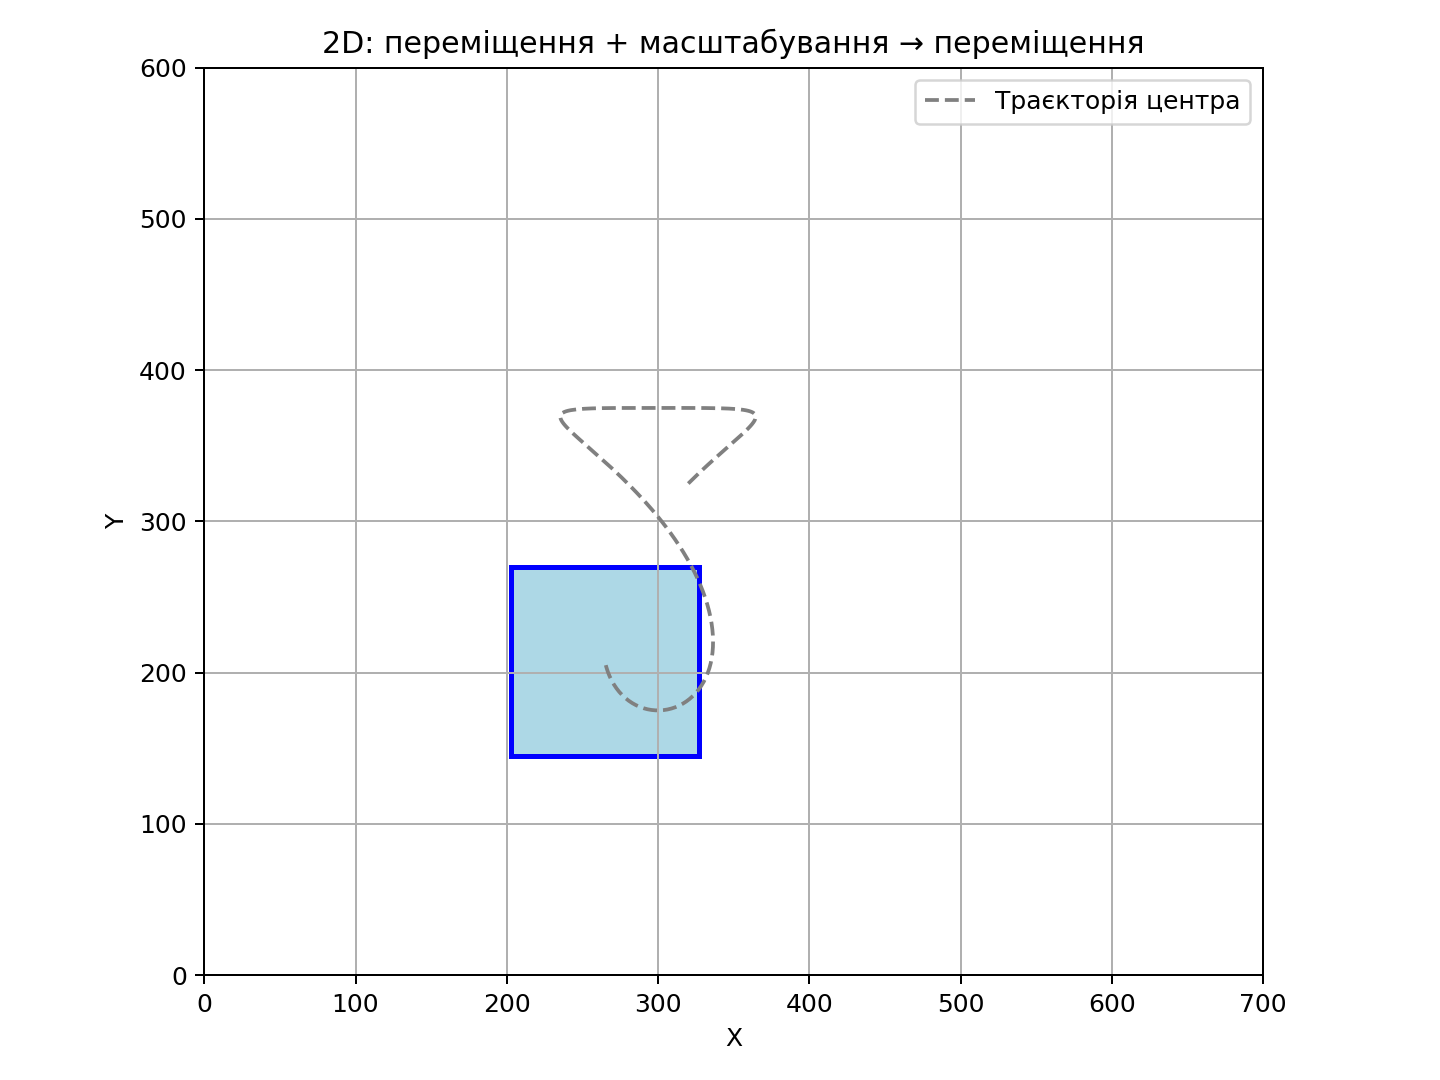
\includegraphics[width=0.85\textwidth]{media/2d_result.png}
  \caption{Результат 2D-перетворень і траєкторія квадрата}
\end{figure}

\begin{figure}[H]
  \centering
  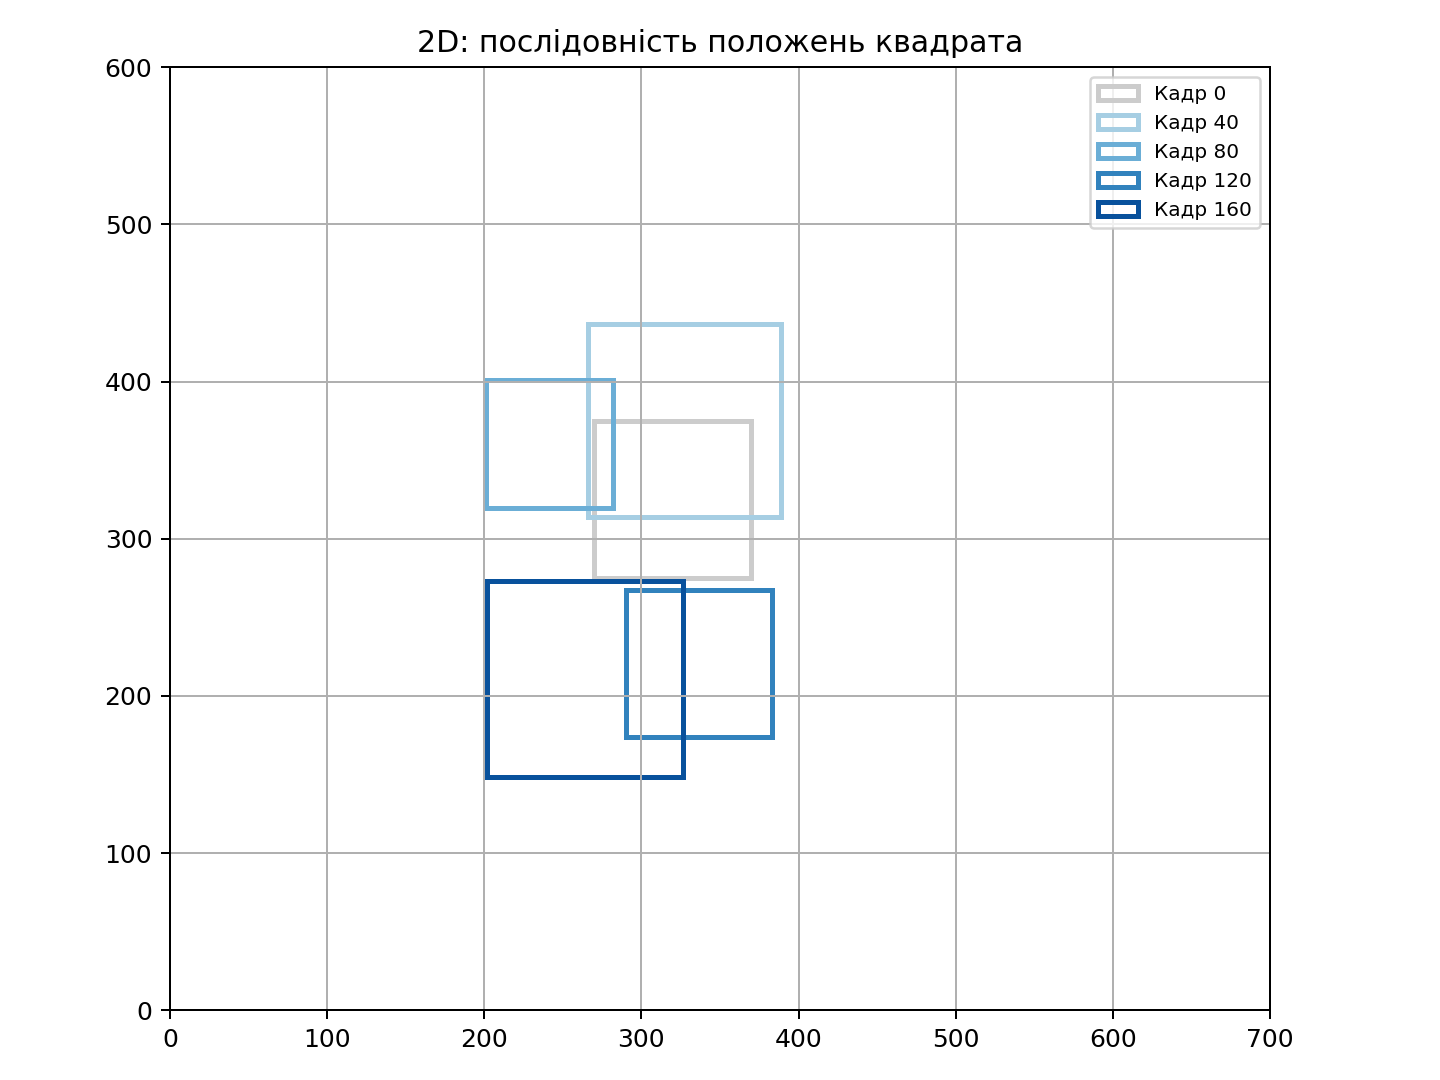
\includegraphics[width=0.85\textwidth]{media/2d_sequence.png}
  \caption{Послідовність положень квадрата у різних кадрах}
\end{figure}

У 3D-частині піраміда складається з квадратної основи та чотирьох бічних граней. Після нахилу та проекції просторові координати відображаються на площині екрана.

\begin{figure}[H]
  \centering
  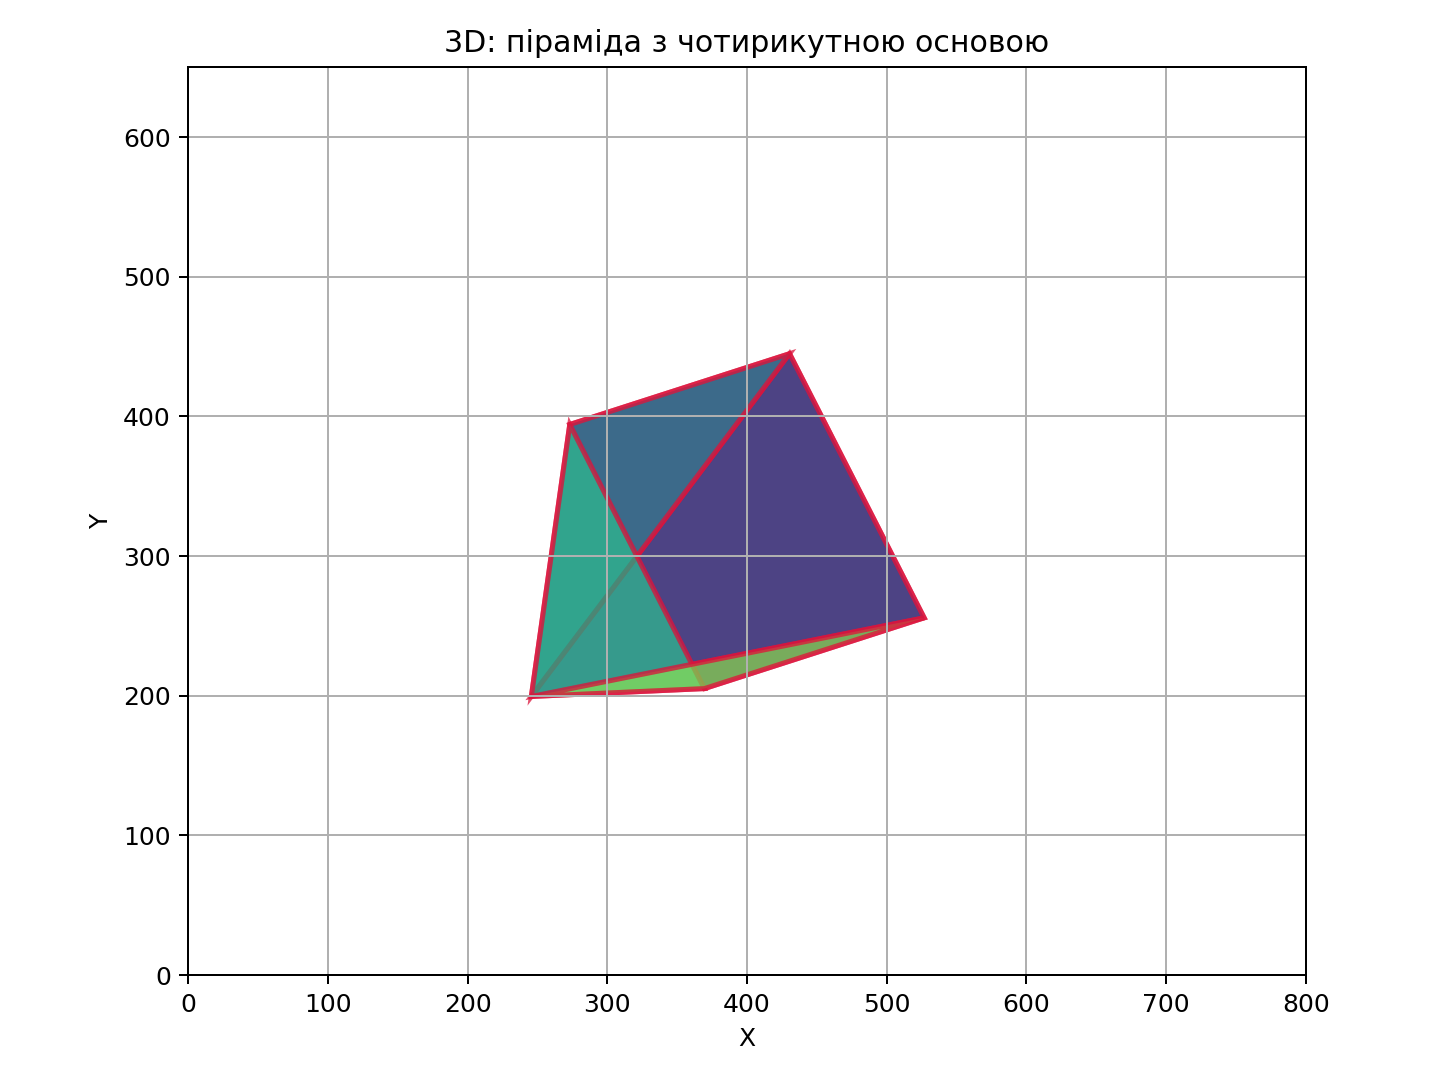
\includegraphics[width=0.82\textwidth]{media/3d_result.png}
  \caption{Аксонометрична проекція піраміди}
\end{figure}

\begin{figure}[H]
  \centering
  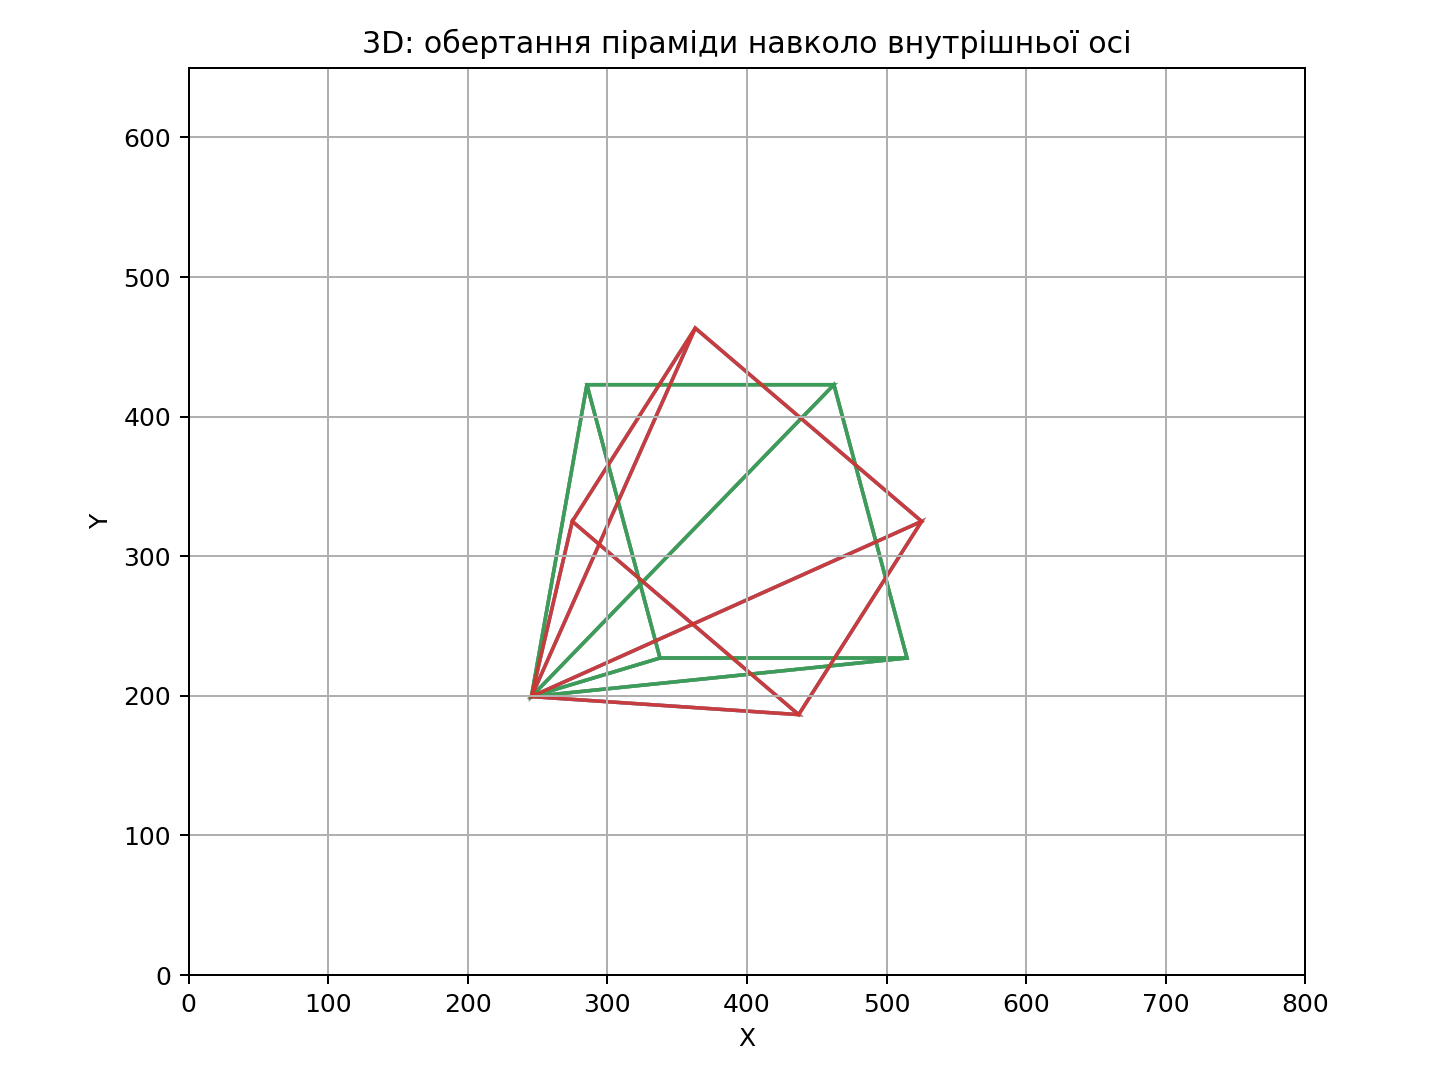
\includegraphics[width=0.82\textwidth]{media/3d_sequence.png}
  \caption{Різні положення піраміди під час обертання}
\end{figure}

\section{Фрагменти програмного коду}

Нижче наведено повний код обох програм лабораторної роботи.

\textbf{Лістинг 1 --- повний програмний код 2D-частини}

\inputminted{python}{../2D.py}

\textbf{Лістинг 2 --- повний програмний код 3D-частини}

\inputminted{python}{../3D.py}

\section{Тестування та верифікація}

Виконано синтаксичну перевірку Python-файлів та контрольний запуск математичних функцій. Матриця квадрата має розмір \(3\times4\), матриця піраміди --- \(4\times5\). Перевірено, що переміщення не змінює форму квадрата, масштабування виконується відносно центра, усі грані піраміди використовують спільні перетворені вершини, а проекція повертає координати, придатні для малювання на 2D-площині.

\begin{itemize}[leftmargin=*,itemsep=0.25em]
  \item 2D-анімація повторюється циклічно, а траєкторія центра залишається видимою.
  \item 3D-піраміда циклічно обертається навколо внутрішньої осі.
  \item Прозорість піраміди змінюється від майже невидимого до повністю видимого стану.
  \item Колір контуру та заливки змінюється протягом анімації.
  \item Об’єкти залишаються в межах заданого графічного вікна.
\end{itemize}

\section{Висновки}

У лабораторній роботі досліджено задання вершин геометричних об’єктів за допомогою розширених координат і матричних перетворень. Для 2D-об’єкта реалізовано послідовність переміщення, масштабування навколо центра та повторного переміщення з відображенням траєкторії. Для 3D-об’єкта побудовано піраміду з чотирикутною основою, виконано обертання навколо внутрішньої осі та аксонометричну проекцію на площину екрана. Додатково реалізовано циклічну зміну прозорості, кольору контуру та кольору заливки. Отримані результати підтверджують коректність використання однорідних матриць для композиції геометричних перетворень.

\end{document}
